\documentclass[11pt,border=5pt]{standalone}
\usepackage{fontspec}
\setmainfont{cmunrm.otf}[BoldFont=cmunbx.otf,ItalicFont=cmunti.otf,BoldItalicFont=cmunbi.otf]
\usepackage{amsmath}
\usepackage{unicode-math}
\setmathfont{NewCMMath-Regular.otf}
\usepackage{tikz}
\usetikzlibrary{arrows.meta,patterns,angles,quotes}
\begin{document}
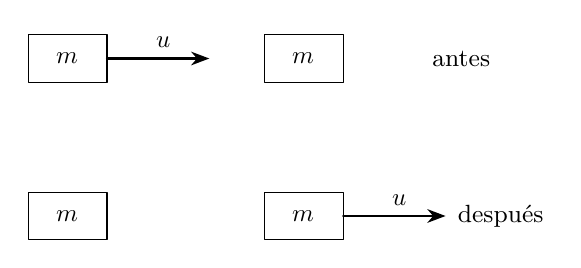
\begin{tikzpicture}[>=Stealth,font=\small,line cap=round,line join=round]
\draw[fill=white] (-2.5,0.7) rectangle (-1.5,1.3);
\node at (-2,1) {$m$};
\draw[fill=white] (0.5,0.7) rectangle (1.5,1.3);
\node at (1,1) {$m$};
\draw[->,thick] (-1.5,1) -- (-0.2,1) node[pos=0.55,above] {$u$};
\node at (3,1) {antes};
\draw[fill=white] (-2.5,-1.3) rectangle (-1.5,-0.7);
\node at (-2,-1) {$m$};
\draw[fill=white] (0.5,-1.3) rectangle (1.5,-0.7);
\node at (1,-1) {$m$};
\draw[->,thick] (1.5,-1) -- (2.8,-1) node[pos=0.55,above] {$u$};
\node at (3.5,-1) {después};

\end{tikzpicture}
\end{document}
